% Options for packages loaded elsewhere
% Options for packages loaded elsewhere
\PassOptionsToPackage{unicode}{hyperref}
\PassOptionsToPackage{hyphens}{url}
\PassOptionsToPackage{dvipsnames,svgnames,x11names}{xcolor}
%
\documentclass[
  spanish,
  a4paper,
  DIV=11,
  numbers=noendperiod]{scrreprt}
\usepackage{xcolor}
\usepackage[top=22mm,bottom=22mm,left=24mm,right=24mm]{geometry}
\usepackage{amsmath,amssymb}
\setcounter{secnumdepth}{5}
\usepackage{iftex}
\ifPDFTeX
  \usepackage[T1]{fontenc}
  \usepackage[utf8]{inputenc}
  \usepackage{textcomp} % provide euro and other symbols
\else % if luatex or xetex
  \usepackage{unicode-math} % this also loads fontspec
  \defaultfontfeatures{Scale=MatchLowercase}
  \defaultfontfeatures[\rmfamily]{Ligatures=TeX,Scale=1}
\fi
\usepackage{lmodern}
\ifPDFTeX\else
  % xetex/luatex font selection
\fi
% Use upquote if available, for straight quotes in verbatim environments
\IfFileExists{upquote.sty}{\usepackage{upquote}}{}
\IfFileExists{microtype.sty}{% use microtype if available
  \usepackage[]{microtype}
  \UseMicrotypeSet[protrusion]{basicmath} % disable protrusion for tt fonts
}{}
\makeatletter
\@ifundefined{KOMAClassName}{% if non-KOMA class
  \IfFileExists{parskip.sty}{%
    \usepackage{parskip}
  }{% else
    \setlength{\parindent}{0pt}
    \setlength{\parskip}{6pt plus 2pt minus 1pt}}
}{% if KOMA class
  \KOMAoptions{parskip=half}}
\makeatother
% Make \paragraph and \subparagraph free-standing
\makeatletter
\ifx\paragraph\undefined\else
  \let\oldparagraph\paragraph
  \renewcommand{\paragraph}{
    \@ifstar
      \xxxParagraphStar
      \xxxParagraphNoStar
  }
  \newcommand{\xxxParagraphStar}[1]{\oldparagraph*{#1}\mbox{}}
  \newcommand{\xxxParagraphNoStar}[1]{\oldparagraph{#1}\mbox{}}
\fi
\ifx\subparagraph\undefined\else
  \let\oldsubparagraph\subparagraph
  \renewcommand{\subparagraph}{
    \@ifstar
      \xxxSubParagraphStar
      \xxxSubParagraphNoStar
  }
  \newcommand{\xxxSubParagraphStar}[1]{\oldsubparagraph*{#1}\mbox{}}
  \newcommand{\xxxSubParagraphNoStar}[1]{\oldsubparagraph{#1}\mbox{}}
\fi
\makeatother

\usepackage{color}
\usepackage{fancyvrb}
\newcommand{\VerbBar}{|}
\newcommand{\VERB}{\Verb[commandchars=\\\{\}]}
\DefineVerbatimEnvironment{Highlighting}{Verbatim}{commandchars=\\\{\}}
% Add ',fontsize=\small' for more characters per line
\usepackage{framed}
\definecolor{shadecolor}{RGB}{241,243,245}
\newenvironment{Shaded}{\begin{snugshade}}{\end{snugshade}}
\newcommand{\AlertTok}[1]{\textcolor[rgb]{0.68,0.00,0.00}{#1}}
\newcommand{\AnnotationTok}[1]{\textcolor[rgb]{0.37,0.37,0.37}{#1}}
\newcommand{\AttributeTok}[1]{\textcolor[rgb]{0.40,0.45,0.13}{#1}}
\newcommand{\BaseNTok}[1]{\textcolor[rgb]{0.68,0.00,0.00}{#1}}
\newcommand{\BuiltInTok}[1]{\textcolor[rgb]{0.00,0.23,0.31}{#1}}
\newcommand{\CharTok}[1]{\textcolor[rgb]{0.13,0.47,0.30}{#1}}
\newcommand{\CommentTok}[1]{\textcolor[rgb]{0.37,0.37,0.37}{#1}}
\newcommand{\CommentVarTok}[1]{\textcolor[rgb]{0.37,0.37,0.37}{\textit{#1}}}
\newcommand{\ConstantTok}[1]{\textcolor[rgb]{0.56,0.35,0.01}{#1}}
\newcommand{\ControlFlowTok}[1]{\textcolor[rgb]{0.00,0.23,0.31}{\textbf{#1}}}
\newcommand{\DataTypeTok}[1]{\textcolor[rgb]{0.68,0.00,0.00}{#1}}
\newcommand{\DecValTok}[1]{\textcolor[rgb]{0.68,0.00,0.00}{#1}}
\newcommand{\DocumentationTok}[1]{\textcolor[rgb]{0.37,0.37,0.37}{\textit{#1}}}
\newcommand{\ErrorTok}[1]{\textcolor[rgb]{0.68,0.00,0.00}{#1}}
\newcommand{\ExtensionTok}[1]{\textcolor[rgb]{0.00,0.23,0.31}{#1}}
\newcommand{\FloatTok}[1]{\textcolor[rgb]{0.68,0.00,0.00}{#1}}
\newcommand{\FunctionTok}[1]{\textcolor[rgb]{0.28,0.35,0.67}{#1}}
\newcommand{\ImportTok}[1]{\textcolor[rgb]{0.00,0.46,0.62}{#1}}
\newcommand{\InformationTok}[1]{\textcolor[rgb]{0.37,0.37,0.37}{#1}}
\newcommand{\KeywordTok}[1]{\textcolor[rgb]{0.00,0.23,0.31}{\textbf{#1}}}
\newcommand{\NormalTok}[1]{\textcolor[rgb]{0.00,0.23,0.31}{#1}}
\newcommand{\OperatorTok}[1]{\textcolor[rgb]{0.37,0.37,0.37}{#1}}
\newcommand{\OtherTok}[1]{\textcolor[rgb]{0.00,0.23,0.31}{#1}}
\newcommand{\PreprocessorTok}[1]{\textcolor[rgb]{0.68,0.00,0.00}{#1}}
\newcommand{\RegionMarkerTok}[1]{\textcolor[rgb]{0.00,0.23,0.31}{#1}}
\newcommand{\SpecialCharTok}[1]{\textcolor[rgb]{0.37,0.37,0.37}{#1}}
\newcommand{\SpecialStringTok}[1]{\textcolor[rgb]{0.13,0.47,0.30}{#1}}
\newcommand{\StringTok}[1]{\textcolor[rgb]{0.13,0.47,0.30}{#1}}
\newcommand{\VariableTok}[1]{\textcolor[rgb]{0.07,0.07,0.07}{#1}}
\newcommand{\VerbatimStringTok}[1]{\textcolor[rgb]{0.13,0.47,0.30}{#1}}
\newcommand{\WarningTok}[1]{\textcolor[rgb]{0.37,0.37,0.37}{\textit{#1}}}

\usepackage{longtable,booktabs,array}
\newcounter{none} % for unnumbered tables
\usepackage{calc} % for calculating minipage widths
% Correct order of tables after \paragraph or \subparagraph
\usepackage{etoolbox}
\makeatletter
\patchcmd\longtable{\par}{\if@noskipsec\mbox{}\fi\par}{}{}
\makeatother
% Allow footnotes in longtable head/foot
\IfFileExists{footnotehyper.sty}{\usepackage{footnotehyper}}{\usepackage{footnote}}
\makesavenoteenv{longtable}
\usepackage{graphicx}
\makeatletter
\newsavebox\pandoc@box
\newcommand*\pandocbounded[1]{% scales image to fit in text height/width
  \sbox\pandoc@box{#1}%
  \Gscale@div\@tempa{\textheight}{\dimexpr\ht\pandoc@box+\dp\pandoc@box\relax}%
  \Gscale@div\@tempb{\linewidth}{\wd\pandoc@box}%
  \ifdim\@tempb\p@<\@tempa\p@\let\@tempa\@tempb\fi% select the smaller of both
  \ifdim\@tempa\p@<\p@\scalebox{\@tempa}{\usebox\pandoc@box}%
  \else\usebox{\pandoc@box}%
  \fi%
}
% Set default figure placement to htbp
\def\fps@figure{htbp}
\makeatother


% definitions for citeproc citations
\NewDocumentCommand\citeproctext{}{}
\NewDocumentCommand\citeproc{mm}{%
  \begingroup\def\citeproctext{#2}\cite{#1}\endgroup}
\makeatletter
 % allow citations to break across lines
 \let\@cite@ofmt\@firstofone
 % avoid brackets around text for \cite:
 \def\@biblabel#1{}
 \def\@cite#1#2{{#1\if@tempswa , #2\fi}}
\makeatother
\newlength{\cslhangindent}
\setlength{\cslhangindent}{1.5em}
\newlength{\csllabelwidth}
\setlength{\csllabelwidth}{3em}
\newenvironment{CSLReferences}[2] % #1 hanging-indent, #2 entry-spacing
 {\begin{list}{}{%
  \setlength{\itemindent}{0pt}
  \setlength{\leftmargin}{0pt}
  \setlength{\parsep}{0pt}
  % turn on hanging indent if param 1 is 1
  \ifodd #1
   \setlength{\leftmargin}{\cslhangindent}
   \setlength{\itemindent}{-1\cslhangindent}
  \fi
  % set entry spacing
  \setlength{\itemsep}{#2\baselineskip}}}
 {\end{list}}
\usepackage{calc}
\newcommand{\CSLBlock}[1]{\hfill\break\parbox[t]{\linewidth}{\strut\ignorespaces#1\strut}}
\newcommand{\CSLLeftMargin}[1]{\parbox[t]{\csllabelwidth}{\strut#1\strut}}
\newcommand{\CSLRightInline}[1]{\parbox[t]{\linewidth - \csllabelwidth}{\strut#1\strut}}
\newcommand{\CSLIndent}[1]{\hspace{\cslhangindent}#1}

\ifLuaTeX
\usepackage[bidi=basic,shorthands=off]{babel}
\else
\usepackage[bidi=default,shorthands=off]{babel}
\fi
\ifLuaTeX
  \usepackage{selnolig} % disable illegal ligatures
\fi


\setlength{\emergencystretch}{3em} % prevent overfull lines

\providecommand{\tightlist}{%
  \setlength{\itemsep}{0pt}\setlength{\parskip}{0pt}}



 


% Estilo LaTeX para el tutorial SBVI
\usepackage{booktabs}
\usepackage{longtable}
\usepackage{array}
\usepackage{tabularx}
\usepackage{ragged2e}
\usepackage{microtype}
\usepackage{fancyhdr}
\usepackage[most]{tcolorbox}
\usepackage{enumitem}
\usepackage{tikz}
\usetikzlibrary{arrows.meta,positioning,shapes.geometric}
\usepackage{siunitx}
\usepackage{xcolor}
\usepackage{titlesec}
\usepackage{hyperref}

\definecolor{BioBlue}{HTML}{17365D}
\definecolor{BioTeal}{HTML}{1F6E78}
\definecolor{BioLight}{HTML}{EEF4F7}
\definecolor{BioGray}{HTML}{5C6770}
\definecolor{BioWarn}{HTML}{8A4B08}
\definecolor{BioRed}{HTML}{8B1E2D}
\definecolor{BioGreen}{HTML}{2F6B4F}

\hypersetup{
  colorlinks=true,
  linkcolor=BioBlue,
  urlcolor=BioTeal,
  citecolor=BioGreen
}

\pagestyle{fancy}
\fancyhf{}
\fancyhead[L]{\small Señales Bioeléctricas y Visualización Interactiva}
\fancyhead[R]{\small sEMG y monitoreo post-ictus}
\fancyfoot[C]{\thepage}
\renewcommand{\headrulewidth}{0.4pt}

\titleformat{\chapter}[display]
  {\bfseries\Huge\color{BioBlue}}
  {\filleft\Large\color{BioTeal}\chaptertitlename\ \thechapter}
  {1ex}
  {\titlerule\vspace{1ex}\filright}
  [\vspace{1ex}\titlerule]

\titleformat{\section}
  {\Large\bfseries\color{BioBlue}}
  {\thesection}{0.7em}{}
\titleformat{\subsection}
  {\large\bfseries\color{BioTeal}}
  {\thesubsection}{0.7em}{}

\newtcolorbox{clinicalbox}[1][]{
  enhanced,
  breakable,
  colback=BioLight,
  colframe=BioBlue,
  boxrule=0.8pt,
  arc=2mm,
  left=2mm,right=2mm,top=1.5mm,bottom=1.5mm,
  title=Solicitud clínica,
  fonttitle=\bfseries,
  #1
}

\newtcolorbox{engineeringbox}[1][]{
  enhanced,
  breakable,
  colback=white,
  colframe=BioTeal,
  boxrule=0.8pt,
  arc=2mm,
  left=2mm,right=2mm,top=1.5mm,bottom=1.5mm,
  title=Decisión de ingeniería,
  fonttitle=\bfseries,
  #1
}

\newtcolorbox{warningbox}[1][]{
  enhanced,
  breakable,
  colback=yellow!4,
  colframe=BioWarn,
  boxrule=0.8pt,
  arc=2mm,
  left=2mm,right=2mm,top=1.5mm,bottom=1.5mm,
  title=Advertencia metodológica,
  fonttitle=\bfseries,
  #1
}

\newtcolorbox{checkpointbox}[1][]{
  enhanced,
  breakable,
  colback=green!3,
  colframe=BioGreen,
  boxrule=0.8pt,
  arc=2mm,
  left=2mm,right=2mm,top=1.5mm,bottom=1.5mm,
  title=Punto de verificación,
  fonttitle=\bfseries,
  #1
}

\setlist[itemize]{topsep=3pt,itemsep=2pt}
\setlist[enumerate]{topsep=3pt,itemsep=2pt}
\renewcommand{\arraystretch}{1.15}
\KOMAoption{captions}{tableheading}
\makeatletter
\@ifpackageloaded{tcolorbox}{}{\usepackage[skins,breakable]{tcolorbox}}
\@ifpackageloaded{fontawesome5}{}{\usepackage{fontawesome5}}
\definecolor{quarto-callout-color}{HTML}{909090}
\definecolor{quarto-callout-note-color}{HTML}{0758E5}
\definecolor{quarto-callout-important-color}{HTML}{CC1914}
\definecolor{quarto-callout-warning-color}{HTML}{EB9113}
\definecolor{quarto-callout-tip-color}{HTML}{00A047}
\definecolor{quarto-callout-caution-color}{HTML}{FC5300}
\definecolor{quarto-callout-color-frame}{HTML}{acacac}
\definecolor{quarto-callout-note-color-frame}{HTML}{4582ec}
\definecolor{quarto-callout-important-color-frame}{HTML}{d9534f}
\definecolor{quarto-callout-warning-color-frame}{HTML}{f0ad4e}
\definecolor{quarto-callout-tip-color-frame}{HTML}{02b875}
\definecolor{quarto-callout-caution-color-frame}{HTML}{fd7e14}
\makeatother
\makeatletter
\@ifpackageloaded{caption}{}{\usepackage{caption}}
\AtBeginDocument{%
\ifdefined\contentsname
  \renewcommand*\contentsname{Tabla de contenidos}
\else
  \newcommand\contentsname{Tabla de contenidos}
\fi
\ifdefined\listfigurename
  \renewcommand*\listfigurename{Listado de Figuras}
\else
  \newcommand\listfigurename{Listado de Figuras}
\fi
\ifdefined\listtablename
  \renewcommand*\listtablename{Listado de Tablas}
\else
  \newcommand\listtablename{Listado de Tablas}
\fi
\ifdefined\figurename
  \renewcommand*\figurename{Figura}
\else
  \newcommand\figurename{Figura}
\fi
\ifdefined\tablename
  \renewcommand*\tablename{Tabla}
\else
  \newcommand\tablename{Tabla}
\fi
}
\@ifpackageloaded{float}{}{\usepackage{float}}
\floatstyle{ruled}
\@ifundefined{c@chapter}{\newfloat{codelisting}{h}{lop}}{\newfloat{codelisting}{h}{lop}[chapter]}
\floatname{codelisting}{Listado}
\newcommand*\listoflistings{\listof{codelisting}{Listado de Listados}}
\makeatother
\makeatletter
\makeatother
\makeatletter
\@ifpackageloaded{caption}{}{\usepackage{caption}}
\@ifpackageloaded{subcaption}{}{\usepackage{subcaption}}
\makeatother
\makeatletter
\@ifpackageloaded{tcolorbox}{}{\usepackage[skins,breakable]{tcolorbox}}
\makeatother
\makeatletter
\@ifundefined{shadecolor}{\definecolor{shadecolor}{HTML}{1F6E78}}{}
\makeatother
\makeatletter
\makeatother
\makeatletter
\ifdefined\Shaded\renewenvironment{Shaded}{\begin{tcolorbox}[borderline west={3pt}{0pt}{shadecolor}, boxrule=0pt, breakable, enhanced, frame hidden, interior hidden, sharp corners]}{\end{tcolorbox}}\fi
\makeatother
\usepackage{bookmark}
\IfFileExists{xurl.sty}{\usepackage{xurl}}{} % add URL line breaks if available
\urlstyle{same}
\hypersetup{
  pdftitle={Tutorial: diseño de un dashboard clínico con sEMG},
  pdfauthor={Señales Bioeléctricas y Visualización Interactiva},
  pdflang={es},
  colorlinks=true,
  linkcolor={blue},
  filecolor={Maroon},
  citecolor={Blue},
  urlcolor={Blue},
  pdfcreator={LaTeX via pandoc}}


\title{Tutorial: diseño de un dashboard clínico con sEMG}
\usepackage{etoolbox}
\makeatletter
\providecommand{\subtitle}[1]{% add subtitle to \maketitle
  \apptocmd{\@title}{\par {\large #1 \par}}{}{}
}
\makeatother
\subtitle{Monitoreo de alteraciones neuromusculares post-ictus con datos
abiertos de PhysioNet}
\author{Señales Bioeléctricas y Visualización Interactiva}
\date{2026-09-18}
\begin{document}
\maketitle

\renewcommand*\contentsname{Tabla de contenidos}
{
\setcounter{tocdepth}{2}
\tableofcontents
}

\begin{tcolorbox}[enhanced jigsaw, arc=.35mm, bottomrule=.15mm, bottomtitle=1mm, breakable, colback=white, colbacktitle=quarto-callout-note-color!10!white, colframe=quarto-callout-note-color-frame, coltitle=black, left=2mm, leftrule=.75mm, opacityback=0, opacitybacktitle=0.6, rightrule=.15mm, title=\textcolor{quarto-callout-note-color}{\faInfo}\hspace{0.5em}{Solicitud clínica}, titlerule=0mm, toprule=.15mm, toptitle=1mm]

Un médico fisiatra solicita una herramienta para
\textbf{monitorear la actividad muscular de personas con antecedente de ictus isquémico},
con énfasis en hemiparesia y uso funcional del músculo durante
actividades de la vida diaria. El médico no solicita un clasificador
automático ni una herramienta de diagnóstico. Solicita un tablero que
responda cuatro preguntas: \textbf{(1)} ¿hay actividad muscular
registrable?, \textbf{(2)} ¿cómo se distribuye esa actividad en el
tiempo?, \textbf{(3)} ¿la calidad del registro permite interpretar los
indicadores con confianza?, y \textbf{(4)} en evaluaciones repetidas y
estandarizadas, ¿existen cambios en la activación neuromuscular
compatibles con evolución de la función motora post-ictus?

\end{tcolorbox}

\chapter{Propósito del tutorial}\label{propuxf3sito-del-tutorial}

Este tutorial guía la construcción de un dashboard clínico a partir de
\textbf{electromiografía de superficie (sEMG)}. El caso de estudio es el
monitoreo post-ictus y el conjunto de datos base es \textbf{Cerebral
Vasoregulation in Elderly with Stroke (CVES)} de PhysioNet
(\citeproc{ref-physionet_cves}{Novak 2018}).

El objetivo no es producir un biomarcador diagnóstico. El objetivo es
diseñar una cadena reproducible que conecte:

\begin{enumerate}
\def\labelenumi{\arabic{enumi}.}
\tightlist
\item
  fisiopatología post-ictus;
\item
  variable fisiológica observable;
\item
  señal bioeléctrica;
\item
  procesamiento digital;
\item
  indicador cuantitativo;
\item
  visualización clínicamente interpretable.
\end{enumerate}

\begin{figure}[H]

{\centering 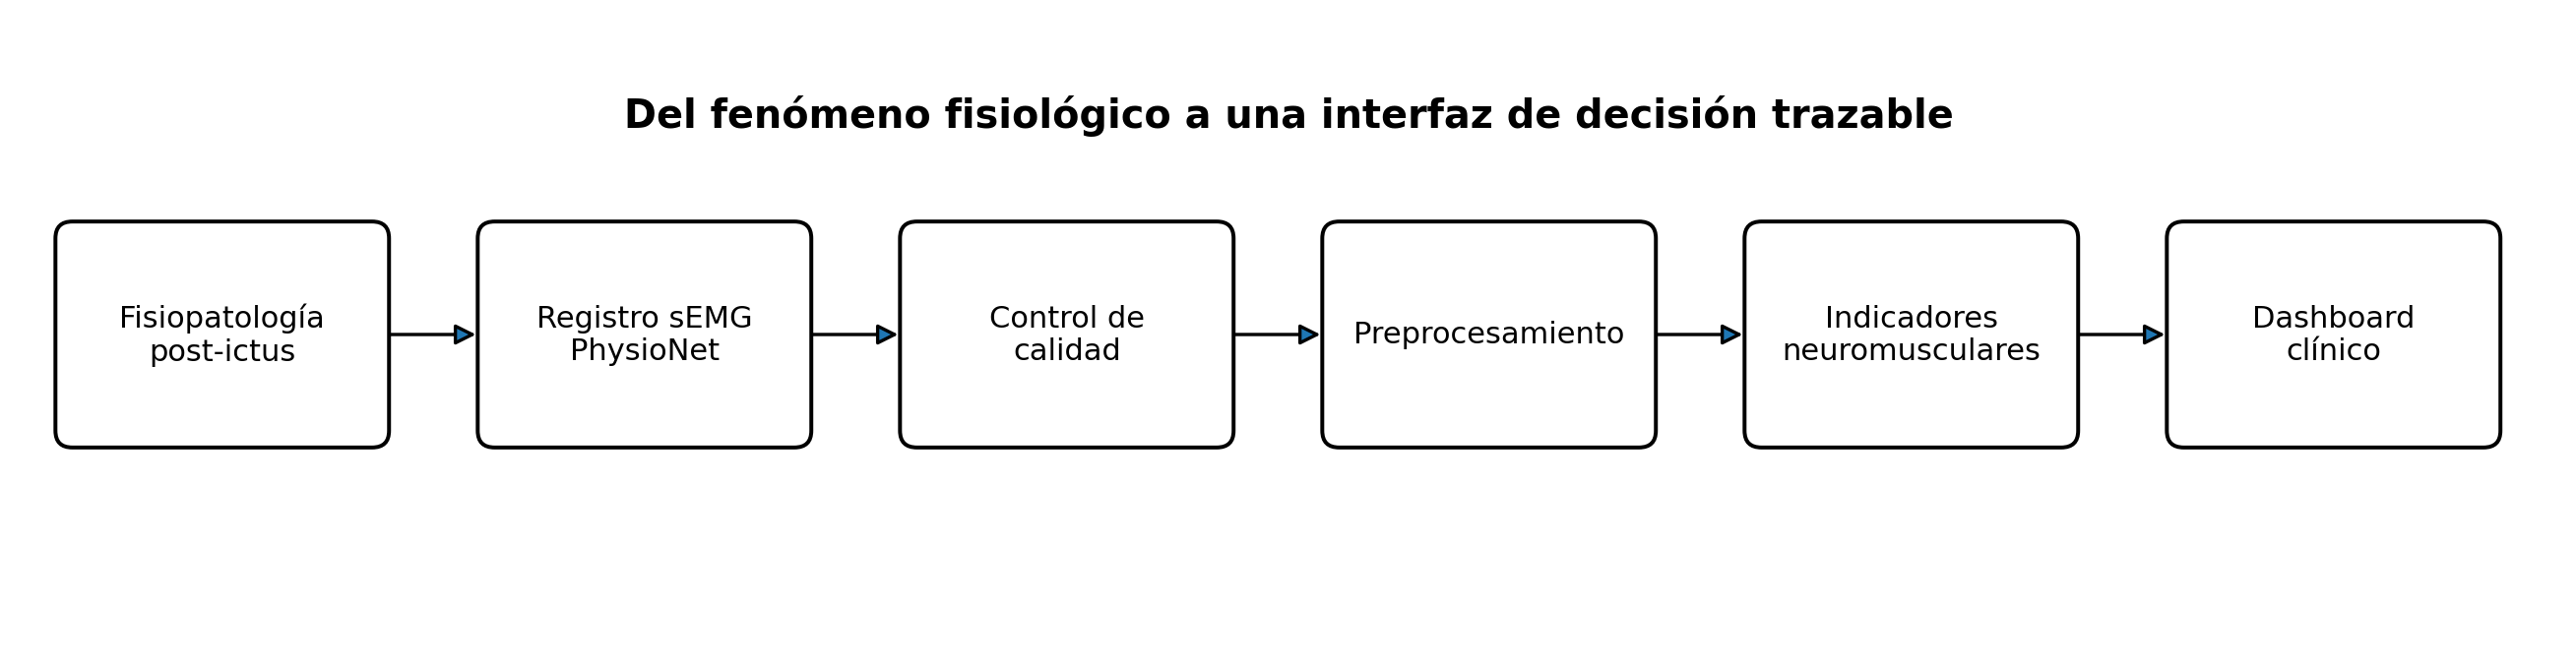
\includegraphics[width=0.96\linewidth,height=\textheight,keepaspectratio]{figuras/pipeline_semg.png}

}

\caption{Pipeline conceptual del tutorial}

\end{figure}%

Al finalizar, el estudiante debe poder justificar \textbf{por qué
calcula cada indicador}, \textbf{qué supuestos necesita} y \textbf{qué
no puede concluir} a partir de la señal.

\section{Resultado esperado}\label{resultado-esperado}

El producto final consta de dos artefactos:

\begin{itemize}
\tightlist
\item
  un \textbf{pipeline de procesamiento} de sEMG reproducible en Python;
\item
  un \textbf{dashboard en Streamlit} que permita explorar segmentos del
  registro, visualizar señal cruda/filtrada/envolvente, inspeccionar
  indicadores y revisar la calidad de señal.
\end{itemize}

\chapter{1. Del problema clínico a una variable
medible}\label{del-problema-cluxednico-a-una-variable-medible}

\section{1.1 ¿Qué cambia después de un
ictus?}\label{quuxe9-cambia-despuuxe9s-de-un-ictus}

Un ictus puede alterar la salida motora descendente y, con ello, la
activación voluntaria del músculo. En rehabilitación post-ictus, la sEMG
es útil porque ofrece información objetiva sobre \textbf{presencia,
intensidad relativa y temporalidad de la activación muscular}, incluso
cuando el movimiento visible es pequeño
(\citeproc{ref-munoznovoa2022}{Muñoz-Novoa et~al. 2022}).

Para este tutorial nos interesan cuatro manifestaciones funcionales:

\begin{itemize}
\tightlist
\item
  reducción o intermitencia de la actividad muscular;
\item
  menor tiempo de participación activa del músculo;
\item
  organización temporal anormal de los episodios de activación;
\item
  posible asimetría entre canales equivalentes, \textbf{solo si la
  identidad anatómica y la lateralidad de los canales están
  documentadas}.
\end{itemize}

\begin{tcolorbox}[enhanced jigsaw, arc=.35mm, bottomrule=.15mm, bottomtitle=1mm, breakable, colback=white, colbacktitle=quarto-callout-warning-color!10!white, colframe=quarto-callout-warning-color-frame, coltitle=black, left=2mm, leftrule=.75mm, opacityback=0, opacitybacktitle=0.6, rightrule=.15mm, title=\textcolor{quarto-callout-warning-color}{\faExclamationTriangle}\hspace{0.5em}{Advertencia metodológica}, titlerule=0mm, toprule=.15mm, toptitle=1mm]

La sEMG \textbf{no mide fuerza directamente}. La amplitud depende, entre
otros factores, del reclutamiento de unidades motoras, la posición del
electrodo, la impedancia piel-electrodo, el tejido subcutáneo y la
geometría del músculo. Por ello, una diferencia de amplitud entre
sujetos no debe interpretarse automáticamente como una diferencia de
fuerza.

\end{tcolorbox}

\section{1.2 Cadena fisiología →
ingeniería}\label{cadena-fisiologuxeda-ingenieruxeda}

{\def\LTcaptype{none} % do not increment counter
\begin{longtable}[]{@{}
  >{\raggedright\arraybackslash}p{(\linewidth - 4\tabcolsep) * \real{0.3333}}
  >{\raggedright\arraybackslash}p{(\linewidth - 4\tabcolsep) * \real{0.3333}}
  >{\raggedright\arraybackslash}p{(\linewidth - 4\tabcolsep) * \real{0.3333}}@{}}
\toprule\noalign{}
\begin{minipage}[b]{\linewidth}\raggedright
Nivel
\end{minipage} & \begin{minipage}[b]{\linewidth}\raggedright
Pregunta
\end{minipage} & \begin{minipage}[b]{\linewidth}\raggedright
Variable/decisión
\end{minipage} \\
\midrule\noalign{}
\endhead
\bottomrule\noalign{}
\endlastfoot
Fisiología & ¿Existe activación neuromuscular? & Actividad eléctrica
muscular registrable \\
Adquisición & ¿La señal contiene información interpretable? & sEMG en
µV, frecuencia de muestreo, artefactos \\
Procesamiento & ¿Cómo se aísla la banda útil? & Filtrado, rectificación,
RMS/envolvente \\
Indicador & ¿Cuánta actividad y durante cuánto tiempo? & RMS, porcentaje
de tiempo activo, tasa y duración de episodios \\
Calidad & ¿Los indicadores son confiables? & Relación de ruido de red,
artefacto de baja frecuencia, datos faltantes \\
Interfaz & ¿Puede el clínico comprenderlo? & Trazado + indicadores +
contexto + advertencias \\
\end{longtable}
}

\chapter{2. Dataset: PhysioNet CVES}\label{dataset-physionet-cves}

El recurso CVES contiene datos multimodales de adultos mayores con
antecedente de ictus isquémico y controles
(\citeproc{ref-novak2010}{Novak et~al. 2010};
\citeproc{ref-physionet_cves}{Novak 2018}). Entre sus archivos existen
registros de ECG, EMG y acelerometría de larga duración. PhysioNet
documenta que los registros de 24 horas de ECG/EMG fueron adquiridos con
un sistema \textbf{ME6000} a \textbf{1000 Hz} y se distribuyen en
formato WFDB (\citeproc{ref-physionet_cves}{Novak 2018}).

El sistema ME6000 está diseñado para adquisición de señales de EMG de
superficie; por ello, este tutorial trata esos canales como sEMG. No
obstante, la interpretación anatómica específica exige revisar la
documentación de adquisición del estudio.

\section{2.1 Por qué este dataset es útil para
docencia}\label{por-quuxe9-este-dataset-es-uxfatil-para-docencia}

\begin{itemize}
\tightlist
\item
  contiene participantes con ictus y controles;
\item
  el registro es suficientemente largo para estudiar actividad muscular
  cotidiana;
\item
  el formato WFDB permite lectura parcial sin descargar decenas de
  gigabytes;
\item
  el archivo \texttt{subjects.csv} incluye variables clínicas como
  grupo, lado del ictus, NIHSS, mRS y síntomas;
\item
  algunos encabezados WFDB contienen cuatro canales \texttt{emg\_0} a
  \texttt{emg\_3}, además de ECG y acelerometría.
\end{itemize}

Como ejemplo didáctico, el sujeto \textbf{S0205} aparece como
participante con ictus, con lateralidad derecha del evento, hemiparesia
izquierda, NIHSS 10 y mRS 3 en la tabla de participantes. Un registro
asociado es \texttt{s0205-05080904}.

\begin{tcolorbox}[enhanced jigsaw, arc=.35mm, bottomrule=.15mm, bottomtitle=1mm, breakable, colback=white, colbacktitle=quarto-callout-warning-color!10!white, colframe=quarto-callout-warning-color-frame, coltitle=black, left=2mm, leftrule=.75mm, opacityback=0, opacitybacktitle=0.6, rightrule=.15mm, title=\textcolor{quarto-callout-warning-color}{\faExclamationTriangle}\hspace{0.5em}{Advertencia metodológica}, titlerule=0mm, toprule=.15mm, toptitle=1mm]

Los nombres \texttt{emg\_0}, \texttt{emg\_1}, etc. no identifican por sí
mismos el músculo ni la lateralidad. Por tanto, el tutorial
\textbf{no asigna nombres anatómicos inventados}. El dashboard mantiene
el identificador original hasta que el estudiante verifique la
correspondencia en el protocolo del estudio.

\end{tcolorbox}

\section{2.2 Acceso reproducible}\label{acceso-reproducible}

Instale Quarto, Python y \texttt{uv}. En la carpeta del proyecto:

\begin{Shaded}
\begin{Highlighting}[]
\ExtensionTok{uv}\NormalTok{ init}
\ExtensionTok{uv}\NormalTok{ add numpy pandas scipy plotly streamlit wfdb pyarrow}
\end{Highlighting}
\end{Shaded}

No descargue el conjunto completo. CVES supera ampliamente lo necesario
para esta práctica. WFDB permite leer únicamente el intervalo
solicitado.

\chapter{3. Inspección del participante y del
registro}\label{inspecciuxf3n-del-participante-y-del-registro}

Primero se inspeccionan metadatos. Esta etapa evita que la ingeniería
pierda el contexto clínico.

\begin{Shaded}
\begin{Highlighting}[]
\ImportTok{import}\NormalTok{ pandas }\ImportTok{as}\NormalTok{ pd}

\NormalTok{SUBJECTS\_URL }\OperatorTok{=} \StringTok{"https://physionet.org/files/cves/1.0.0/subjects.csv"}
\NormalTok{subjects }\OperatorTok{=}\NormalTok{ pd.read\_csv(SUBJECTS\_URL)}

\NormalTok{subject\_id }\OperatorTok{=} \StringTok{"S0205"}
\NormalTok{row }\OperatorTok{=}\NormalTok{ subjects.loc[subjects[}\StringTok{"subject\_number"}\NormalTok{].eq(subject\_id)].iloc[}\DecValTok{0}\NormalTok{]}

\NormalTok{cols }\OperatorTok{=}\NormalTok{ [}
    \StringTok{"subject\_number"}\NormalTok{, }\StringTok{"group"}\NormalTok{, }\StringTok{"age"}\NormalTok{, }\StringTok{"gender"}\NormalTok{,}
    \StringTok{"NIHSS"}\NormalTok{, }\StringTok{"MRS"}\NormalTok{, }\StringTok{"Stroke Side"}\NormalTok{, }\StringTok{"Symptoms"}
\NormalTok{]}
\BuiltInTok{print}\NormalTok{(row[cols])}
\end{Highlighting}
\end{Shaded}

Los metadatos observados son:

{\def\LTcaptype{none} % do not increment counter
\begin{longtable}[]{@{}
  >{\raggedright\arraybackslash}p{(\linewidth - 2\tabcolsep) * \real{0.5000}}
  >{\raggedright\arraybackslash}p{(\linewidth - 2\tabcolsep) * \real{0.5000}}@{}}
\toprule\noalign{}
\begin{minipage}[b]{\linewidth}\raggedright
Campo y valor
\end{minipage} & \begin{minipage}[b]{\linewidth}\raggedright
Explicación
\end{minipage} \\
\midrule\noalign{}
\endhead
\bottomrule\noalign{}
\endlastfoot
\textbf{\texttt{subject\_number}}: \texttt{S0205} & Identificador único
del participante dentro del conjunto de datos. Permite relacionar sus
datos clínicos con los registros fisiológicos sin utilizar directamente
información personal identificable. \\
\textbf{\texttt{group}}: \texttt{STROKE} & Grupo clínico al que
pertenece el participante. \texttt{STROKE} indica que corresponde al
grupo de sujetos con antecedente de \textbf{ictus}. \\
\textbf{\texttt{age}}: \texttt{63} & Edad del participante, expresada en
años. En este registro, el sujeto tiene \textbf{63 años}. \\
\textbf{\texttt{gender}}: \texttt{F} & Sexo codificado en el dataset.
\texttt{F} corresponde a \textbf{Female}, es decir, mujer. \\
\textbf{\texttt{NIHSS}}: \texttt{10.0} & Puntaje en la \textbf{National
Institutes of Health Stroke Scale (NIHSS)}. Esta escala cuantifica el
déficit neurológico asociado al ictus. Debe considerarse una variable
clínica externa y no una característica derivada de la sEMG. \\
\textbf{\texttt{MRS}}: \texttt{3.0} & Puntaje en la \textbf{modified
Rankin Scale (mRS)}. Evalúa el nivel global de discapacidad o
dependencia funcional después del ictus. Un valor de 3 corresponde a
discapacidad moderada. \\
\textbf{\texttt{Stroke\ Side}}: \texttt{RIGHT} & Indica el lado
reportado en el dataset como asociado al ictus. Es necesario verificar
en la documentación si se refiere al \textbf{hemisferio cerebral
afectado} o al \textbf{lado corporal comprometido} antes de utilizar
esta variable en análisis de lateralidad de sEMG. \\
\textbf{\texttt{Symptoms}}: \texttt{L\ hemiparesis} & Síntoma clínico
registrado. \texttt{L\ hemiparesis} significa \textbf{hemiparesia
izquierda}, es decir, debilidad motora parcial del lado izquierdo del
cuerpo. \\
\textbf{\texttt{Name}}: \texttt{47} & Índice de la fila en la estructura
de datos de Pandas. \textbf{No corresponde a una variable clínica} del
participante. \\
\textbf{\texttt{dtype}}: \texttt{object} & Tipo de dato de la
\texttt{Series} de Pandas. \textbf{No corresponde a una variable
clínica}. \\
\end{longtable}
}

A continuación se inspecciona el encabezado del registro sin descargar
el archivo completo:

\begin{Shaded}
\begin{Highlighting}[]
\ImportTok{import}\NormalTok{ wfdb}

\NormalTok{PN\_DIR }\OperatorTok{=} \StringTok{"cves/1.0.0/data/24h{-}electromyography"}
\NormalTok{RECORD }\OperatorTok{=} \StringTok{"s0205{-}05080904"}

\NormalTok{header }\OperatorTok{=}\NormalTok{ wfdb.rdheader(RECORD, pn\_dir}\OperatorTok{=}\NormalTok{PN\_DIR)}
\BuiltInTok{print}\NormalTok{(}\StringTok{"fs ="}\NormalTok{, header.fs)}
\BuiltInTok{print}\NormalTok{(}\StringTok{"duración [h] ="}\NormalTok{, header.sig\_len }\OperatorTok{/}\NormalTok{ header.fs }\OperatorTok{/} \DecValTok{3600}\NormalTok{)}
\BuiltInTok{print}\NormalTok{(}\StringTok{"canales ="}\NormalTok{, header.sig\_name)}
\end{Highlighting}
\end{Shaded}

El estudiante debe verificar tres cosas antes de procesar:

\begin{enumerate}
\def\labelenumi{\arabic{enumi}.}
\tightlist
\item
  frecuencia de muestreo;
\item
  unidades;
\item
  lista de canales disponibles.
\end{enumerate}

\begin{tcolorbox}[enhanced jigsaw, arc=.35mm, bottomrule=.15mm, bottomtitle=1mm, breakable, colback=white, colbacktitle=quarto-callout-important-color!10!white, colframe=quarto-callout-important-color-frame, coltitle=black, left=2mm, leftrule=.75mm, opacityback=0, opacitybacktitle=0.6, rightrule=.15mm, title=\textcolor{quarto-callout-important-color}{\faExclamation}\hspace{0.5em}{Punto de verificación}, titlerule=0mm, toprule=.15mm, toptitle=1mm]

Si el encabezado no contiene canales EMG o la unidad no es
interpretable, el pipeline debe detenerse. Un dashboard no corrige un
problema semántico de los datos.

\end{tcolorbox}

\chapter{4. Selección eficiente de un
segmento}\label{selecciuxf3n-eficiente-de-un-segmento}

Para una primera exploración no es necesario cargar horas de señal.
Comience con 120 s.

\begin{Shaded}
\begin{Highlighting}[]
\ImportTok{import}\NormalTok{ numpy }\ImportTok{as}\NormalTok{ np}

\NormalTok{START\_S }\OperatorTok{=} \DecValTok{0}
\NormalTok{DURATION\_S }\OperatorTok{=} \DecValTok{120}

\NormalTok{emg\_idx }\OperatorTok{=}\NormalTok{ [}
\NormalTok{    i }\ControlFlowTok{for}\NormalTok{ i, name }\KeywordTok{in} \BuiltInTok{enumerate}\NormalTok{(header.sig\_name)}
    \ControlFlowTok{if} \StringTok{"emg"} \KeywordTok{in}\NormalTok{ name.lower()}
\NormalTok{]}

\NormalTok{record }\OperatorTok{=}\NormalTok{ wfdb.rdrecord(}
\NormalTok{    RECORD,}
\NormalTok{    pn\_dir}\OperatorTok{=}\NormalTok{PN\_DIR,}
\NormalTok{    sampfrom}\OperatorTok{=}\BuiltInTok{int}\NormalTok{(START\_S }\OperatorTok{*}\NormalTok{ header.fs),}
\NormalTok{    sampto}\OperatorTok{=}\BuiltInTok{int}\NormalTok{((START\_S }\OperatorTok{+}\NormalTok{ DURATION\_S) }\OperatorTok{*}\NormalTok{ header.fs),}
\NormalTok{    channels}\OperatorTok{=}\NormalTok{emg\_idx,}
\NormalTok{)}

\NormalTok{fs }\OperatorTok{=} \BuiltInTok{float}\NormalTok{(record.fs)}
\NormalTok{x }\OperatorTok{=}\NormalTok{ record.p\_signal}
\NormalTok{names }\OperatorTok{=}\NormalTok{ record.sig\_name}

\BuiltInTok{print}\NormalTok{(x.shape)}
\BuiltInTok{print}\NormalTok{(names)}
\end{Highlighting}
\end{Shaded}

\section{4.1 ¿Por qué trabajar por
ventanas?}\label{por-quuxe9-trabajar-por-ventanas}

La sEMG de actividades diarias es no estacionaria. Un indicador global
de varias horas puede ocultar episodios cortos de actividad. Por ello se
combinan dos escalas:

\begin{itemize}
\tightlist
\item
  \textbf{escala de señal:} milisegundos a segundos, para filtrar y
  estimar amplitud;
\item
  \textbf{escala funcional:} segundos a minutos, para resumir actividad
  y presentarla en el dashboard.
\end{itemize}

\chapter{5. Control de calidad antes del indicador
clínico}\label{control-de-calidad-antes-del-indicador-cluxednico}

El error habitual es filtrar y calcular RMS sin preguntarse si la señal
es confiable. El orden correcto es:

\[
\text{dato crudo} \rightarrow \text{calidad} \rightarrow \text{preprocesamiento} \rightarrow \text{indicador}
\]

\section{5.1 Indicadores de calidad
propuestos}\label{indicadores-de-calidad-propuestos}

\subsection{Potencia alrededor de la red
eléctrica}\label{potencia-alrededor-de-la-red-eluxe9ctrica}

En el contexto del registro realizado en Estados Unidos, 60 Hz es una
frecuencia esperable de interferencia eléctrica. Se estima la fracción
de potencia alrededor de 60 Hz respecto a la potencia total entre 20 y
450 Hz.

\[
Q_{60}=100\frac{\sum_{f\in[59,61]}P(f)}{\sum_{f\in[20,450]}P(f)}
\]

No existe un umbral universal. El valor se usa para \textbf{comparación
interna y detección de segmentos sospechosos}, no como criterio clínico
absoluto.

\subsection{Artefacto de baja
frecuencia}\label{artefacto-de-baja-frecuencia}

Movimiento del electrodo y cambios de contacto pueden aumentar energía a
muy baja frecuencia. Una razón exploratoria es:

\[
Q_{LF}=100\frac{\sum_{f\in[0.5,15]}P(f)}{\sum_{f\in[0.5,450]}P(f)}
\]

\section{5.2 Implementación}\label{implementaciuxf3n}

\begin{Shaded}
\begin{Highlighting}[]
\ImportTok{from}\NormalTok{ scipy }\ImportTok{import}\NormalTok{ signal}


\KeywordTok{def}\NormalTok{ band\_power\_ratio(x, fs, num\_band, den\_band):}
\NormalTok{    f, pxx }\OperatorTok{=}\NormalTok{ signal.welch(x, fs}\OperatorTok{=}\NormalTok{fs, nperseg}\OperatorTok{=}\BuiltInTok{min}\NormalTok{(}\BuiltInTok{len}\NormalTok{(x), }\BuiltInTok{int}\NormalTok{(}\DecValTok{4} \OperatorTok{*}\NormalTok{ fs)))}

\NormalTok{    num }\OperatorTok{=}\NormalTok{ (f }\OperatorTok{\textgreater{}=}\NormalTok{ num\_band[}\DecValTok{0}\NormalTok{]) }\OperatorTok{\&}\NormalTok{ (f }\OperatorTok{\textless{}=}\NormalTok{ num\_band[}\DecValTok{1}\NormalTok{])}
\NormalTok{    den }\OperatorTok{=}\NormalTok{ (f }\OperatorTok{\textgreater{}=}\NormalTok{ den\_band[}\DecValTok{0}\NormalTok{]) }\OperatorTok{\&}\NormalTok{ (f }\OperatorTok{\textless{}=}\NormalTok{ den\_band[}\DecValTok{1}\NormalTok{])}

\NormalTok{    p\_num }\OperatorTok{=}\NormalTok{ np.trapz(pxx[num], f[num])}
\NormalTok{    p\_den }\OperatorTok{=}\NormalTok{ np.trapz(pxx[den], f[den])}
    \ControlFlowTok{return}\NormalTok{ np.nan }\ControlFlowTok{if}\NormalTok{ p\_den }\OperatorTok{\textless{}=} \DecValTok{0} \ControlFlowTok{else} \DecValTok{100} \OperatorTok{*}\NormalTok{ p\_num }\OperatorTok{/}\NormalTok{ p\_den}


\NormalTok{quality }\OperatorTok{=}\NormalTok{ []}
\ControlFlowTok{for}\NormalTok{ j, name }\KeywordTok{in} \BuiltInTok{enumerate}\NormalTok{(names):}
\NormalTok{    sig }\OperatorTok{=}\NormalTok{ x[:, j]}
\NormalTok{    quality.append(\{}
        \StringTok{"channel"}\NormalTok{: name,}
        \StringTok{"line\_noise\_60\_pct"}\NormalTok{: band\_power\_ratio(sig, fs, (}\DecValTok{59}\NormalTok{, }\DecValTok{61}\NormalTok{), (}\DecValTok{20}\NormalTok{, }\DecValTok{450}\NormalTok{)),}
        \StringTok{"low\_freq\_pct"}\NormalTok{: band\_power\_ratio(sig, fs, (}\FloatTok{0.5}\NormalTok{, }\DecValTok{15}\NormalTok{), (}\FloatTok{0.5}\NormalTok{, }\DecValTok{450}\NormalTok{)),}
        \StringTok{"missing\_pct"}\NormalTok{: }\DecValTok{100} \OperatorTok{*}\NormalTok{ np.mean(}\OperatorTok{\textasciitilde{}}\NormalTok{np.isfinite(sig)),}
\NormalTok{    \})}

\NormalTok{quality\_df }\OperatorTok{=}\NormalTok{ pd.DataFrame(quality)}
\NormalTok{quality\_df}
\end{Highlighting}
\end{Shaded}

\chapter{6. Preprocesamiento de sEMG}\label{preprocesamiento-de-semg}

\section{6.1 Banda de interés}\label{banda-de-interuxe9s}

Para esta práctica se usa un filtro pasabanda \textbf{20--450 Hz}. La
elección se justifica por dos razones:

\begin{itemize}
\tightlist
\item
  atenuar deriva y artefactos lentos;
\item
  conservar la mayor parte del contenido útil de sEMG sin acercarse
  demasiado a Nyquist, que para 1000 Hz es 500 Hz.
\end{itemize}

El límite superior no es una propiedad universal del músculo. Depende
del sistema de adquisición, frecuencia de muestreo y ancho de banda real
del sensor.

\section{6.2 ¿Rectificación o RMS?}\label{rectificaciuxf3n-o-rms}

La señal EMG bipolar oscila alrededor de cero. Para estimar magnitud de
activación se usa una transformación no negativa. Dos opciones
frecuentes son:

\begin{itemize}
\tightlist
\item
  rectificación + filtro pasa-bajas para envolvente;
\item
  RMS en ventana móvil.
\end{itemize}

En este tutorial se conservan ambas porque responden preguntas
diferentes: la envolvente es útil para visualizar el perfil temporal y
RMS es conveniente para resumir magnitud local.

\section{6.3 Código de procesamiento}\label{cuxf3digo-de-procesamiento}

\begin{Shaded}
\begin{Highlighting}[]
\ImportTok{from}\NormalTok{ scipy }\ImportTok{import}\NormalTok{ signal}
\ImportTok{from}\NormalTok{ scipy.ndimage }\ImportTok{import}\NormalTok{ uniform\_filter1d}


\KeywordTok{def}\NormalTok{ interpolate\_nan(x):}
\NormalTok{    x }\OperatorTok{=}\NormalTok{ np.asarray(x, dtype}\OperatorTok{=}\BuiltInTok{float}\NormalTok{)}
    \ControlFlowTok{if}\NormalTok{ np.}\BuiltInTok{all}\NormalTok{(np.isfinite(x)):}
        \ControlFlowTok{return}\NormalTok{ x}
\NormalTok{    idx }\OperatorTok{=}\NormalTok{ np.arange(}\BuiltInTok{len}\NormalTok{(x))}
\NormalTok{    good }\OperatorTok{=}\NormalTok{ np.isfinite(x)}
    \ControlFlowTok{if}\NormalTok{ good.}\BuiltInTok{sum}\NormalTok{() }\OperatorTok{\textless{}} \DecValTok{2}\NormalTok{:}
        \ControlFlowTok{return}\NormalTok{ np.full\_like(x, np.nan)}
    \ControlFlowTok{return}\NormalTok{ np.interp(idx, idx[good], x[good])}


\KeywordTok{def}\NormalTok{ bandpass\_semg(x, fs, low}\OperatorTok{=}\FloatTok{20.0}\NormalTok{, high}\OperatorTok{=}\FloatTok{450.0}\NormalTok{, order}\OperatorTok{=}\DecValTok{4}\NormalTok{):}
\NormalTok{    x }\OperatorTok{=}\NormalTok{ interpolate\_nan(x)}
\NormalTok{    sos }\OperatorTok{=}\NormalTok{ signal.butter(order, [low, high], btype}\OperatorTok{=}\StringTok{"bandpass"}\NormalTok{, fs}\OperatorTok{=}\NormalTok{fs, output}\OperatorTok{=}\StringTok{"sos"}\NormalTok{)}
    \ControlFlowTok{return}\NormalTok{ signal.sosfiltfilt(sos, x)}


\KeywordTok{def}\NormalTok{ notch\_if\_needed(x, fs, f0}\OperatorTok{=}\FloatTok{60.0}\NormalTok{, q}\OperatorTok{=}\FloatTok{30.0}\NormalTok{):}
\NormalTok{    b, a }\OperatorTok{=}\NormalTok{ signal.iirnotch(f0, q, fs}\OperatorTok{=}\NormalTok{fs)}
    \ControlFlowTok{return}\NormalTok{ signal.filtfilt(b, a, x)}


\KeywordTok{def}\NormalTok{ rms\_envelope(x, fs, window\_ms}\OperatorTok{=}\DecValTok{250}\NormalTok{):}
\NormalTok{    n }\OperatorTok{=} \BuiltInTok{max}\NormalTok{(}\DecValTok{3}\NormalTok{, }\BuiltInTok{int}\NormalTok{(window\_ms }\OperatorTok{/} \DecValTok{1000} \OperatorTok{*}\NormalTok{ fs))}
    \ControlFlowTok{return}\NormalTok{ np.sqrt(uniform\_filter1d(x}\OperatorTok{**}\DecValTok{2}\NormalTok{, size}\OperatorTok{=}\NormalTok{n, mode}\OperatorTok{=}\StringTok{"nearest"}\NormalTok{))}


\KeywordTok{def}\NormalTok{ linear\_envelope(x, fs, cutoff}\OperatorTok{=}\FloatTok{5.0}\NormalTok{):}
\NormalTok{    rect }\OperatorTok{=}\NormalTok{ np.}\BuiltInTok{abs}\NormalTok{(x)}
\NormalTok{    sos }\OperatorTok{=}\NormalTok{ signal.butter(}\DecValTok{4}\NormalTok{, cutoff, btype}\OperatorTok{=}\StringTok{"lowpass"}\NormalTok{, fs}\OperatorTok{=}\NormalTok{fs, output}\OperatorTok{=}\StringTok{"sos"}\NormalTok{)}
    \ControlFlowTok{return}\NormalTok{ signal.sosfiltfilt(sos, rect)}
\end{Highlighting}
\end{Shaded}

\begin{tcolorbox}[enhanced jigsaw, arc=.35mm, bottomrule=.15mm, bottomtitle=1mm, breakable, colback=white, colbacktitle=quarto-callout-tip-color!10!white, colframe=quarto-callout-tip-color-frame, coltitle=black, left=2mm, leftrule=.75mm, opacityback=0, opacitybacktitle=0.6, rightrule=.15mm, title=\textcolor{quarto-callout-tip-color}{\faLightbulb}\hspace{0.5em}{Decisión de ingeniería}, titlerule=0mm, toprule=.15mm, toptitle=1mm]

No aplique el notch de 60 Hz automáticamente. Primero observe el
espectro o el indicador de ruido. El filtrado excesivo puede modificar
información útil y crear una falsa sensación de limpieza.

\end{tcolorbox}

\chapter{7. De la señal a indicadores de
monitoreo}\label{de-la-seuxf1al-a-indicadores-de-monitoreo}

\section{7.1 Indicador 1: RMS local}\label{indicador-1-rms-local}

Para una ventana de \(N\) muestras:

\[
\mathrm{RMS}=\sqrt{\frac{1}{N}\sum_{n=1}^{N}x^2[n]}
\]

En sEMG, RMS resume la magnitud de la señal en una ventana local. En
este tutorial se usa una ventana de \textbf{250 ms} para el tablero. Esa
duración produce una curva más estable que la señal cruda y mantiene
resolución suficiente para actividades cotidianas relativamente lentas.

\textbf{Interpretación:} mayor RMS significa mayor magnitud eléctrica
registrada, no necesariamente mayor fuerza.

\section{7.2 Indicador 2: fracción de tiempo
activo}\label{indicador-2-fracciuxf3n-de-tiempo-activo}

Se define un umbral interno sobre la serie RMS. Como el dataset no
contiene una contracción voluntaria máxima estandarizada para
normalización, se evita reportar \texttt{\%MVC}.

Se usa un umbral robusto exploratorio:

\begin{enumerate}
\def\labelenumi{\arabic{enumi}.}
\tightlist
\item
  tomar el 20 \% de valores RMS más bajos;
\item
  estimar mediana y MAD;
\item
  definir \(T=\mathrm{mediana}+3\,\mathrm{MAD}_{esc}\).
\end{enumerate}

\[
\mathrm{MAD}_{esc}=1.4826\,\mathrm{median}(|x-\mathrm{median}(x)|)
\]

La fracción activa es:

\[
A=100\frac{N(RMS>T)}{N_{total}}
\]

Este indicador responde: \textbf{¿qué porcentaje del segmento presenta
actividad por encima del nivel basal interno?}

\section{7.3 Indicador 3: tasa de episodios de
activación}\label{indicador-3-tasa-de-episodios-de-activaciuxf3n}

Una transición de inactivo a activo inicia un episodio. Se reporta:

\[
R_b=\frac{N_{episodios}}{\text{duración en minutos}}
\]

Este indicador describe \textbf{fragmentación temporal} de la
activación.

\section{7.4 Indicador 4: duración mediana de
episodios}\label{indicador-4-duraciuxf3n-mediana-de-episodios}

La duración de cada episodio se calcula a partir de la señal binaria de
actividad. Se reporta mediana, no media, porque los episodios largos
pueden sesgar la distribución.

\section{7.5 Indicador 5: cambio longitudinal de RMS durante
actividad}\label{indicador-5-cambio-longitudinal-de-rms-durante-actividad}

Para seguimiento de rehabilitación interesa separar la \textbf{magnitud
de activación durante los periodos realmente activos} de la cantidad de
tiempo en que el músculo permanece inactivo. Para una sesión clínica
\(k\), se define primero:

\[
RMS_{act,k}=\operatorname{mediana}\{RMS[n]\;|\;RMS[n]>T_k\}
\]

donde \(T_k\) es el umbral de actividad calculado con el mismo
procedimiento en todas las visitas. Tomando la primera evaluación
estandarizada como referencia:

\[
\Delta RMS_{rel,k}=100\frac{RMS_{act,k}-RMS_{act,0}}{RMS_{act,0}}
\]

Este indicador resume el \textbf{cambio porcentual de la magnitud
eléctrica durante activaciones detectadas}. En un estudio piloto de
seguimiento post-ictus, el RMS aumentó en la mayoría de los músculos
paréticos después de rehabilitación, por lo que puede aportar
información complementaria para monitorizar cambios neuromusculares
(\citeproc{ref-zhu2020}{Zhu et~al. 2020}).

\textbf{Interpretación longitudinal:} un aumento de \(\Delta RMS_{rel}\)
puede ser compatible con mayor capacidad de activación/reclutamiento
durante una tarea comparable, pero \textbf{no demuestra por sí solo
recuperación neurológica ni aumento de fuerza}.

\begin{tcolorbox}[enhanced jigsaw, arc=.35mm, bottomrule=.15mm, bottomtitle=1mm, breakable, colback=white, colbacktitle=quarto-callout-warning-color!10!white, colframe=quarto-callout-warning-color-frame, coltitle=black, left=2mm, leftrule=.75mm, opacityback=0, opacitybacktitle=0.6, rightrule=.15mm, title=\textcolor{quarto-callout-warning-color}{\faExclamationTriangle}\hspace{0.5em}{Advertencia metodológica}, titlerule=0mm, toprule=.15mm, toptitle=1mm]

El RMS entre visitas solo es interpretable si se controla el músculo
registrado, posición de electrodos, preparación de piel, ganancia,
tarea, postura, carga, ventana RMS y filtros. Si estas condiciones
cambian, la variación instrumental puede ser del mismo orden o mayor que
el cambio fisiológico.

\end{tcolorbox}

\section{7.6 Indicador 6: distancia relativa de frecuencia mediana
respecto al músculo
contralateral}\label{indicador-6-distancia-relativa-de-frecuencia-mediana-respecto-al-muxfasculo-contralateral}

La \textbf{frecuencia mediana (MDF)} divide en dos partes iguales la
potencia espectral dentro de la banda de análisis:

\[
\int_{f_L}^{MDF}P(f)\,df
=
\frac{1}{2}\int_{f_L}^{f_H}P(f)\,df
\]

con \(f_L=20\,\mathrm{Hz}\) y \(f_H=450\,\mathrm{Hz}\) en este tutorial.
Cuando se dispone de un par de músculos homólogos paretico/contralateral
correctamente identificado, se propone:

\[
D_{MDF,k}=100\frac{|MDF_{paretico,k}-MDF_{contra,k}|}{MDF_{contra,k}}
\]

El indicador no busca que MDF aumente o disminuya en una dirección
universal; busca cuantificar \textbf{cuán distante está el patrón
espectral del músculo parético respecto a una referencia contralateral
del mismo sujeto}. En el seguimiento piloto de Zhu et al., la MDF del
músculo parético tendió a aproximarse al valor contralateral durante la
rehabilitación (\citeproc{ref-zhu2020}{Zhu et~al. 2020}). Por tanto, una
reducción de \(D_{MDF}\), bajo un protocolo repetido y controlado, puede
considerarse compatible con convergencia del comportamiento espectral.

\begin{tcolorbox}[enhanced jigsaw, arc=.35mm, bottomrule=.15mm, bottomtitle=1mm, breakable, colback=white, colbacktitle=quarto-callout-warning-color!10!white, colframe=quarto-callout-warning-color-frame, coltitle=black, left=2mm, leftrule=.75mm, opacityback=0, opacitybacktitle=0.6, rightrule=.15mm, title=\textcolor{quarto-callout-warning-color}{\faExclamationTriangle}\hspace{0.5em}{Advertencia metodológica}, titlerule=0mm, toprule=.15mm, toptitle=1mm]

CVES es un estudio transversal y el registro de 24 h de EMG corresponde
al día 1 (\citeproc{ref-physionet_cves}{Novak 2018}). Además, los
canales aparecen como \texttt{emg\_0}, \texttt{emg\_1}, etc., sin
identificación anatómica suficiente en el encabezado. En consecuencia,
el dataset permite enseñar el cálculo de MDF por canal, pero
\textbf{no permite afirmar una trayectoria de recuperación} ni calcular
\(D_{MDF}\) como indicador clínico hasta verificar músculo, lateralidad
y disponer de visitas repetidas comparables.

\end{tcolorbox}

\section{7.7 Indicadores que NO se calculan
automáticamente}\label{indicadores-que-no-se-calculan-automuxe1ticamente}

\textbf{Asimetría bilateral.} Solo es válida si existe certeza de que
dos canales representan el mismo músculo en lados opuestos.

\textbf{Co-contracción agonista-antagonista.} Es relevante en alteración
motora post-ictus (\citeproc{ref-wang2025}{Wang et~al. 2025}), pero
exige conocer exactamente qué músculos representan los canales. Sin esa
información, calcular un índice de co-contracción sería
metodológicamente incorrecto.

\textbf{Frecuencia mediana como fatiga.} Puede ser útil en contracciones
relativamente estacionarias, pero un registro de vida diaria mezcla
tareas, posturas y niveles de fuerza. No se usa como indicador primario
en este dashboard.

\chapter{8. Funciones para extraer los
indicadores}\label{funciones-para-extraer-los-indicadores}

\begin{Shaded}
\begin{Highlighting}[]
\KeywordTok{def}\NormalTok{ robust\_activity\_threshold(rms):}
\NormalTok{    rms }\OperatorTok{=}\NormalTok{ np.asarray(rms, dtype}\OperatorTok{=}\BuiltInTok{float}\NormalTok{)}
\NormalTok{    q20 }\OperatorTok{=}\NormalTok{ np.nanquantile(rms, }\FloatTok{0.20}\NormalTok{)}
\NormalTok{    base }\OperatorTok{=}\NormalTok{ rms[rms }\OperatorTok{\textless{}=}\NormalTok{ q20]}
\NormalTok{    med }\OperatorTok{=}\NormalTok{ np.nanmedian(base)}
\NormalTok{    mad }\OperatorTok{=} \FloatTok{1.4826} \OperatorTok{*}\NormalTok{ np.nanmedian(np.}\BuiltInTok{abs}\NormalTok{(base }\OperatorTok{{-}}\NormalTok{ med))}
    \ControlFlowTok{return}\NormalTok{ med }\OperatorTok{+} \FloatTok{3.0} \OperatorTok{*}\NormalTok{ mad}


\KeywordTok{def}\NormalTok{ run\_lengths(binary, fs):}
\NormalTok{    binary }\OperatorTok{=}\NormalTok{ np.asarray(binary, dtype}\OperatorTok{=}\BuiltInTok{bool}\NormalTok{)}
\NormalTok{    starts }\OperatorTok{=}\NormalTok{ np.flatnonzero(np.diff(np.r\_[}\VariableTok{False}\NormalTok{, binary].astype(}\BuiltInTok{int}\NormalTok{)) }\OperatorTok{==} \DecValTok{1}\NormalTok{)}
\NormalTok{    ends }\OperatorTok{=}\NormalTok{ np.flatnonzero(np.diff(np.r\_[binary, }\VariableTok{False}\NormalTok{].astype(}\BuiltInTok{int}\NormalTok{)) }\OperatorTok{==} \OperatorTok{{-}}\DecValTok{1}\NormalTok{) }\OperatorTok{+} \DecValTok{1}
\NormalTok{    durations }\OperatorTok{=}\NormalTok{ (ends }\OperatorTok{{-}}\NormalTok{ starts) }\OperatorTok{/}\NormalTok{ fs}
    \ControlFlowTok{return}\NormalTok{ starts, ends, durations}


\KeywordTok{def}\NormalTok{ median\_frequency(x, fs, band}\OperatorTok{=}\NormalTok{(}\FloatTok{20.0}\NormalTok{, }\FloatTok{450.0}\NormalTok{)):}
    \CommentTok{"""Frecuencia mediana espectral dentro de una banda definida."""}
\NormalTok{    x }\OperatorTok{=}\NormalTok{ np.asarray(x, dtype}\OperatorTok{=}\BuiltInTok{float}\NormalTok{)}
\NormalTok{    f, pxx }\OperatorTok{=}\NormalTok{ signal.welch(}
\NormalTok{        x,}
\NormalTok{        fs}\OperatorTok{=}\NormalTok{fs,}
\NormalTok{        nperseg}\OperatorTok{=}\BuiltInTok{min}\NormalTok{(}\BuiltInTok{len}\NormalTok{(x), }\BuiltInTok{max}\NormalTok{(}\DecValTok{256}\NormalTok{, }\BuiltInTok{int}\NormalTok{(}\DecValTok{4} \OperatorTok{*}\NormalTok{ fs)))}
\NormalTok{    )}

\NormalTok{    mask }\OperatorTok{=}\NormalTok{ (f }\OperatorTok{\textgreater{}=}\NormalTok{ band[}\DecValTok{0}\NormalTok{]) }\OperatorTok{\&}\NormalTok{ (f }\OperatorTok{\textless{}=}\NormalTok{ band[}\DecValTok{1}\NormalTok{])}
\NormalTok{    fb }\OperatorTok{=}\NormalTok{ f[mask]}
\NormalTok{    pb }\OperatorTok{=}\NormalTok{ pxx[mask]}

    \ControlFlowTok{if} \BuiltInTok{len}\NormalTok{(fb) }\OperatorTok{\textless{}} \DecValTok{2} \KeywordTok{or}\NormalTok{ np.nansum(pb) }\OperatorTok{\textless{}=} \DecValTok{0}\NormalTok{:}
        \ControlFlowTok{return}\NormalTok{ np.nan}

    \CommentTok{\# Integral acumulada por trapecios, sin depender de scipy.integrate.}
\NormalTok{    df }\OperatorTok{=}\NormalTok{ np.diff(fb)}
\NormalTok{    areas }\OperatorTok{=} \FloatTok{0.5} \OperatorTok{*}\NormalTok{ (pb[:}\OperatorTok{{-}}\DecValTok{1}\NormalTok{] }\OperatorTok{+}\NormalTok{ pb[}\DecValTok{1}\NormalTok{:]) }\OperatorTok{*}\NormalTok{ df}
\NormalTok{    cumulative }\OperatorTok{=}\NormalTok{ np.r\_[}\FloatTok{0.0}\NormalTok{, np.cumsum(areas)]}
\NormalTok{    half\_power }\OperatorTok{=} \FloatTok{0.5} \OperatorTok{*}\NormalTok{ cumulative[}\OperatorTok{{-}}\DecValTok{1}\NormalTok{]}
\NormalTok{    idx }\OperatorTok{=} \BuiltInTok{int}\NormalTok{(np.searchsorted(cumulative, half\_power, side}\OperatorTok{=}\StringTok{"left"}\NormalTok{))}
\NormalTok{    idx }\OperatorTok{=} \BuiltInTok{min}\NormalTok{(idx, }\BuiltInTok{len}\NormalTok{(fb) }\OperatorTok{{-}} \DecValTok{1}\NormalTok{)}
    \ControlFlowTok{return} \BuiltInTok{float}\NormalTok{(fb[idx])}


\KeywordTok{def}\NormalTok{ longitudinal\_rms\_change(current\_active\_rms, baseline\_active\_rms):}
    \CommentTok{"""Cambio porcentual de RMS activo respecto a la visita basal."""}
    \ControlFlowTok{if} \KeywordTok{not}\NormalTok{ np.isfinite(baseline\_active\_rms) }\KeywordTok{or}\NormalTok{ baseline\_active\_rms }\OperatorTok{\textless{}=} \DecValTok{0}\NormalTok{:}
        \ControlFlowTok{return}\NormalTok{ np.nan}
    \ControlFlowTok{return} \FloatTok{100.0} \OperatorTok{*}\NormalTok{ (current\_active\_rms }\OperatorTok{{-}}\NormalTok{ baseline\_active\_rms) }\OperatorTok{/}\NormalTok{ baseline\_active\_rms}


\KeywordTok{def}\NormalTok{ mdf\_distance\_to\_contralateral(mdf\_paretic, mdf\_contralateral):}
    \CommentTok{"""Distancia relativa (\%) entre MDF parética y contralateral."""}
    \ControlFlowTok{if} \KeywordTok{not}\NormalTok{ np.isfinite(mdf\_contralateral) }\KeywordTok{or}\NormalTok{ mdf\_contralateral }\OperatorTok{\textless{}=} \DecValTok{0}\NormalTok{:}
        \ControlFlowTok{return}\NormalTok{ np.nan}
    \ControlFlowTok{return} \FloatTok{100.0} \OperatorTok{*} \BuiltInTok{abs}\NormalTok{(mdf\_paretic }\OperatorTok{{-}}\NormalTok{ mdf\_contralateral) }\OperatorTok{/}\NormalTok{ mdf\_contralateral}


\KeywordTok{def}\NormalTok{ semg\_metrics(filtered, fs):}
\NormalTok{    rms }\OperatorTok{=}\NormalTok{ rms\_envelope(filtered, fs, window\_ms}\OperatorTok{=}\DecValTok{250}\NormalTok{)}
\NormalTok{    env }\OperatorTok{=}\NormalTok{ linear\_envelope(filtered, fs, cutoff}\OperatorTok{=}\FloatTok{5.0}\NormalTok{)}
\NormalTok{    thr }\OperatorTok{=}\NormalTok{ robust\_activity\_threshold(rms)}
\NormalTok{    active }\OperatorTok{=}\NormalTok{ rms }\OperatorTok{\textgreater{}}\NormalTok{ thr}

\NormalTok{    starts, ends, durations }\OperatorTok{=}\NormalTok{ run\_lengths(active, fs)}
\NormalTok{    minutes }\OperatorTok{=} \BuiltInTok{len}\NormalTok{(filtered) }\OperatorTok{/}\NormalTok{ fs }\OperatorTok{/} \DecValTok{60}

    \ControlFlowTok{return}\NormalTok{ \{}
        \StringTok{"rms"}\NormalTok{: rms,}
        \StringTok{"envelope"}\NormalTok{: env,}
        \StringTok{"threshold"}\NormalTok{: thr,}
        \StringTok{"active"}\NormalTok{: active,}
        \StringTok{"median\_rms\_uV"}\NormalTok{: }\BuiltInTok{float}\NormalTok{(np.nanmedian(rms)),}
        \StringTok{"active\_rms\_median\_uV"}\NormalTok{: (}
            \BuiltInTok{float}\NormalTok{(np.nanmedian(rms[active])) }\ControlFlowTok{if}\NormalTok{ np.}\BuiltInTok{any}\NormalTok{(active) }\ControlFlowTok{else}\NormalTok{ np.nan}
\NormalTok{        ),}
        \StringTok{"mdf\_hz"}\NormalTok{: median\_frequency(filtered, fs, band}\OperatorTok{=}\NormalTok{(}\FloatTok{20.0}\NormalTok{, }\FloatTok{450.0}\NormalTok{)),}
        \StringTok{"active\_time\_pct"}\NormalTok{: }\BuiltInTok{float}\NormalTok{(}\DecValTok{100} \OperatorTok{*}\NormalTok{ np.nanmean(active)),}
        \StringTok{"bursts\_per\_min"}\NormalTok{: }\BuiltInTok{float}\NormalTok{(}\BuiltInTok{len}\NormalTok{(starts) }\OperatorTok{/}\NormalTok{ minutes) }\ControlFlowTok{if}\NormalTok{ minutes }\OperatorTok{\textgreater{}} \DecValTok{0} \ControlFlowTok{else}\NormalTok{ np.nan,}
        \StringTok{"median\_burst\_s"}\NormalTok{: }\BuiltInTok{float}\NormalTok{(np.nanmedian(durations)) }\ControlFlowTok{if} \BuiltInTok{len}\NormalTok{(durations) }\ControlFlowTok{else} \FloatTok{0.0}\NormalTok{,}
\NormalTok{    \}}
\end{Highlighting}
\end{Shaded}

\section{8.1 Cómo construir la comparación
longitudinal}\label{cuxf3mo-construir-la-comparaciuxf3n-longitudinal}

Los dos indicadores nuevos requieren \textbf{visitas clínicas
repetidas}. La unidad de comparación no debe ser un segmento arbitrario
de 24 horas, sino la misma tarea funcional bajo un protocolo
equivalente. Para cada visita se almacenan, como mínimo:

\begin{itemize}
\tightlist
\item
  participante;
\item
  fecha/visita;
\item
  canal y músculo confirmado;
\item
  lado paretico/contralateral;
\item
  tarea, postura y carga;
\item
  \texttt{active\_rms\_median\_uV};
\item
  \texttt{mdf\_hz};
\item
  escala clínica asociada, si está disponible (por ejemplo, FMA o NIHSS,
  sin convertirla automáticamente en etiqueta de EMG).
\end{itemize}

El cálculo longitudinal puede escribirse así:

\begin{Shaded}
\begin{Highlighting}[]
\KeywordTok{def}\NormalTok{ longitudinal\_pair\_metrics(current, baseline, contralateral}\OperatorTok{=}\VariableTok{None}\NormalTok{):}
\NormalTok{    out }\OperatorTok{=}\NormalTok{ \{}
        \StringTok{"delta\_active\_rms\_pct"}\NormalTok{: longitudinal\_rms\_change(}
\NormalTok{            current[}\StringTok{"active\_rms\_median\_uV"}\NormalTok{],}
\NormalTok{            baseline[}\StringTok{"active\_rms\_median\_uV"}\NormalTok{],}
\NormalTok{        )}
\NormalTok{    \}}

    \ControlFlowTok{if}\NormalTok{ contralateral }\KeywordTok{is} \KeywordTok{not} \VariableTok{None}\NormalTok{:}
\NormalTok{        out[}\StringTok{"mdf\_gap\_pct"}\NormalTok{] }\OperatorTok{=}\NormalTok{ mdf\_distance\_to\_contralateral(}
\NormalTok{            current[}\StringTok{"mdf\_hz"}\NormalTok{],}
\NormalTok{            contralateral[}\StringTok{"mdf\_hz"}\NormalTok{],}
\NormalTok{        )}
    \ControlFlowTok{else}\NormalTok{:}
\NormalTok{        out[}\StringTok{"mdf\_gap\_pct"}\NormalTok{] }\OperatorTok{=}\NormalTok{ np.nan}

    \ControlFlowTok{return}\NormalTok{ out}
\end{Highlighting}
\end{Shaded}

\begin{tcolorbox}[enhanced jigsaw, arc=.35mm, bottomrule=.15mm, bottomtitle=1mm, breakable, colback=white, colbacktitle=quarto-callout-tip-color!10!white, colframe=quarto-callout-tip-color-frame, coltitle=black, left=2mm, leftrule=.75mm, opacityback=0, opacitybacktitle=0.6, rightrule=.15mm, title=\textcolor{quarto-callout-tip-color}{\faLightbulb}\hspace{0.5em}{Decisión de ingeniería}, titlerule=0mm, toprule=.15mm, toptitle=1mm]

Para el dashboard longitudinal, la visualización recomendada es una
serie temporal por visita con dos paneles separados:
\(\Delta RMS_{rel}\) y \(D_{MDF}\). No deben combinarse en un único
``score de recuperación'' porque miden dimensiones diferentes y no
existe una ponderación clínica validada para este tutorial.

\end{tcolorbox}

\chapter{9. Tabla de trazabilidad
fisiológica}\label{tabla-de-trazabilidad-fisioluxf3gica}

El dashboard debe mostrar únicamente métricas con una cadena de
interpretación explícita.

{\def\LTcaptype{none} % do not increment counter
\begin{longtable}[]{@{}
  >{\raggedright\arraybackslash}p{(\linewidth - 6\tabcolsep) * \real{0.2500}}
  >{\raggedright\arraybackslash}p{(\linewidth - 6\tabcolsep) * \real{0.2500}}
  >{\raggedright\arraybackslash}p{(\linewidth - 6\tabcolsep) * \real{0.2500}}
  >{\raggedright\arraybackslash}p{(\linewidth - 6\tabcolsep) * \real{0.2500}}@{}}
\toprule\noalign{}
\begin{minipage}[b]{\linewidth}\raggedright
Indicador
\end{minipage} & \begin{minipage}[b]{\linewidth}\raggedright
Significado ingenieril
\end{minipage} & \begin{minipage}[b]{\linewidth}\raggedright
Relación funcional plausible
\end{minipage} & \begin{minipage}[b]{\linewidth}\raggedright
Riesgo de interpretación
\end{minipage} \\
\midrule\noalign{}
\endhead
\bottomrule\noalign{}
\endlastfoot
RMS local & Magnitud de sEMG en ventana & Nivel relativo de activación &
No equivale a fuerza; sensible a electrodos \\
Tiempo activo & Ocupación temporal sobre umbral & Participación muscular
durante la tarea & Depende del umbral y del segmento \\
Episodios/min & Frecuencia de inicios de actividad & Fragmentación o
recurrencia del uso muscular & Puede reflejar tarea, no patología \\
Duración mediana & Persistencia de episodios & Capacidad de sostener
actividad & Requiere contexto de actividad \\
\(\Delta RMS_{rel}\) & Cambio de RMS activo respecto a visita basal &
Cambio longitudinal de magnitud de activación & Muy sensible a
protocolo/electrodos; no equivale a fuerza \\
\(D_{MDF}\) & Distancia espectral frente a músculo contralateral &
Convergencia del patrón espectral bajo seguimiento & Requiere músculos
homólogos, bilateralidad y tareas comparables \\
Ruido 60 Hz & Contaminación espectral & Ninguna; es calidad de señal &
No es indicador clínico \\
Baja frecuencia & Artefacto lento/movimiento & Ninguna; es calidad de
señal & Movimiento real y artefacto pueden coexistir \\
\end{longtable}
}

\chapter{10. Diseño del dashboard}\label{diseuxf1o-del-dashboard}

El tablero se diseña para responder preguntas clínicas, no para mostrar
todas las variables disponibles.

\section{10.1 Jerarquía visual}\label{jerarquuxeda-visual}

\textbf{Nivel 1 --- Contexto clínico}\\
Participante, grupo, edad, lateralidad del ictus, NIHSS, mRS y síntomas
disponibles.

\textbf{Nivel 2 --- Señal}\\
Trazado crudo, filtrado, envolvente y umbral.

\textbf{Nivel 3 --- Indicadores}\\
Tiempo activo, RMS mediana, episodios/min y duración mediana. En un
protocolo longitudinal: cambio de RMS activo respecto a la visita basal
y distancia relativa de MDF frente al músculo contralateral homólogo.

\textbf{Nivel 4 --- Calidad}\\
Ruido de red, energía de baja frecuencia y faltantes.

\textbf{Nivel 5 --- Limitaciones}\\
Mensaje visible indicando que el dashboard es exploratorio y no
sustituye evaluación clínica.

\section{10.2 Qué evitar}\label{quuxe9-evitar}

\begin{itemize}
\tightlist
\item
  semáforos rojo/verde sin umbrales clínicamente validados;
\item
  un único ``score de salud muscular'' sin modelo validado;
\item
  comparar amplitud absoluta entre pacientes como si fuese fuerza;
\item
  ocultar los filtros aplicados;
\item
  identificar músculos sin evidencia documental;
\item
  convertir correlación en diagnóstico.
\end{itemize}

\chapter{11. Aplicación completa en
Streamlit}\label{aplicaciuxf3n-completa-en-streamlit}

Guarde el siguiente código como \texttt{app\_dashboard\_semg.py}. Una
copia separada se incluye junto con este tutorial.

\begin{Shaded}
\begin{Highlighting}[]
\CommentTok{\# Véase el archivo app\_dashboard\_semg.py incluido con el tutorial.}
\CommentTok{\# En clase se recomienda revisar ese archivo por bloques:}
\CommentTok{\# 1) carga de metadatos;}
\CommentTok{\# 2) lectura parcial WFDB;}
\CommentTok{\# 3) control de calidad;}
\CommentTok{\# 4) preprocesamiento;}
\CommentTok{\# 5) indicadores;}
\CommentTok{\# 6) visualización.}
\end{Highlighting}
\end{Shaded}

Ejecute:

\begin{Shaded}
\begin{Highlighting}[]
\ExtensionTok{uv}\NormalTok{ run streamlit run app\_dashboard\_semg.py}
\end{Highlighting}
\end{Shaded}

\chapter{12. Validación del pipeline}\label{validaciuxf3n-del-pipeline}

\section{12.1 Validación técnica
mínima}\label{validaciuxf3n-tuxe9cnica-muxednima}

Antes de interpretar el dashboard, verifique:

\begin{itemize}
\tightlist
\item
  \texttt{fs} leído del encabezado y no escrito manualmente;
\item
  unidades del canal;
\item
  ausencia de \texttt{NaN} masivos;
\item
  estabilidad del filtro;
\item
  que el espectro post-filtrado no presente energía fuera de la banda
  esperada;
\item
  que el umbral de actividad no marque casi todo el segmento activo o
  inactivo por un fallo numérico;
\item
  que la duración de episodios tenga sentido respecto a la tarea
  observada;
\item
  que el RMS longitudinal se compare únicamente bajo un protocolo de
  adquisición equivalente;
\item
  que MDF se calcule sobre segmentos activos y suficientemente largos
  para una estimación espectral estable;
\item
  que cualquier comparación paretico/contralateral use músculos
  homólogos identificados documentalmente.
\end{itemize}

\section{12.2 Validación
fisiológica}\label{validaciuxf3n-fisioluxf3gica}

La pregunta no es ``¿el gráfico se ve bien?'', sino:

\begin{quote}
¿El indicador conserva una interpretación fisiológica defendible después
de cada transformación?
\end{quote}

Ejemplo: si el RMS aumenta después de aplicar un filtro, esa diferencia
debe explicarse por el cambio en contenido espectral, no asumirse como
mayor activación biológica.

\chapter{13. Actividad práctica
propuesta}\label{actividad-pruxe1ctica-propuesta}

El estudiante debe seleccionar un participante con ictus y uno control,
y para cada uno:

\begin{enumerate}
\def\labelenumi{\arabic{enumi}.}
\tightlist
\item
  inspeccionar metadatos y encabezado WFDB;
\item
  seleccionar tres segmentos de al menos 120 s en momentos diferentes;
\item
  calcular métricas de calidad;
\item
  aplicar el mismo pipeline de preprocesamiento;
\item
  generar indicadores de actividad;
\item
  discutir qué diferencias son atribuibles al sujeto y cuáles pueden
  depender del contexto de registro;
\item
  documentar qué información faltante impide una conclusión clínica más
  fuerte.
\end{enumerate}

No se exige concluir que el sujeto con ictus tiene ``peor'' señal. Se
exige distinguir \textbf{dato}, \textbf{indicador} e
\textbf{interpretación}.

\chapter{14. Preguntas de
verificación}\label{preguntas-de-verificaciuxf3n}

\begin{enumerate}
\def\labelenumi{\arabic{enumi}.}
\tightlist
\item
  ¿Por qué el RMS no debe interpretarse directamente como fuerza
  muscular?
\item
  ¿Qué efecto tendría reducir la ventana RMS de 250 ms a 50 ms?
\item
  ¿Por qué un notch de 60 Hz no debe aplicarse sin revisar primero la
  contaminación espectral?
\item
  ¿Qué información necesita para calcular una asimetría bilateral
  interpretable?
\item
  ¿Por qué la frecuencia mediana no es un indicador primario de fatiga
  en un registro de actividad diaria no controlada?
\item
  ¿Qué ventaja tiene separar indicadores de calidad de los indicadores
  funcionales?
\item
  ¿Qué cambia en la interpretación si el segmento corresponde a reposo,
  marcha o una tarea de miembro superior?
\item
  ¿Por qué un aumento de RMS entre visitas no puede interpretarse
  automáticamente como recuperación motora?
\item
  ¿Qué significa que \(D_{MDF}\) disminuya y qué condiciones deben
  cumplirse antes de interpretarlo?
\item
  ¿Qué evidencia adicional necesitaría para convertir este dashboard en
  una herramienta clínica de seguimiento longitudinal?
\end{enumerate}

\chapter{15. Criterios de aprendizaje}\label{criterios-de-aprendizaje}

Al terminar el tutorial, el estudiante demuestra logro si puede:

\begin{itemize}
\tightlist
\item
  conectar una alteración neuromuscular post-ictus con una variable
  observable en sEMG;
\item
  justificar parámetros de filtrado y ventanas temporales;
\item
  separar métricas de calidad de señal de indicadores fisiológicos;
\item
  implementar lectura parcial de PhysioNet en WFDB;
\item
  construir un dashboard cuyo orden visual siga preguntas clínicas;
\item
  calcular e interpretar un cambio longitudinal de RMS bajo condiciones
  estandarizadas;
\item
  calcular MDF y justificar cuándo puede compararse con el músculo
  contralateral;
\item
  declarar explícitamente las limitaciones que impiden una inferencia
  diagnóstica.
\end{itemize}

\chapter{16. Cierre}\label{cierre}

Un dashboard biomédico no es una colección de gráficas. Es una
\textbf{interfaz de decisión} cuyo valor depende de la trazabilidad
entre fisiología, adquisición, procesamiento e interpretación. En el
caso post-ictus, la sEMG puede aportar una ventana objetiva a la
actividad muscular (\citeproc{ref-munoznovoa2022}{Muñoz-Novoa et~al.
2022}), pero su utilidad depende de no confundir amplitud eléctrica con
fuerza, no inventar la anatomía de los canales y no ocultar la
incertidumbre asociada al registro.

La arquitectura desarrollada aquí puede ampliarse posteriormente con:

\begin{itemize}
\tightlist
\item
  anotaciones de actividad;
\item
  acelerometría sincronizada;
\item
  comparación longitudinal del mismo sujeto mediante
  \(\Delta RMS_{rel}\) y, cuando exista mapeo bilateral confiable,
  \(D_{MDF}\);
\item
  índices bilaterales cuando la lateralidad esté documentada;
\item
  coactivación agonista-antagonista cuando los músculos estén
  identificados;
\item
  análisis por tarea en lugar de análisis por tiempo arbitrario.
\end{itemize}

\chapter{Referencias}\label{referencias}

\protect\phantomsection\label{refs}
\begin{CSLReferences}{1}{1}
\bibitem[\citeproctext]{ref-munoznovoa2022}
Muñoz-Novoa, Maria, Morten B. Kristoffersen, Katharina S. Sunnerhagen,
Annelie Naber, Margit Alt Murphy, y Max Ortiz-Catalan. 2022. {«Upper
Limb Stroke Rehabilitation Using Surface Electromyography: A Systematic
Review and Meta-Analysis»}. \emph{Frontiers in Human Neuroscience} 16:
897870. \url{https://doi.org/10.3389/fnhum.2022.897870}.

\bibitem[\citeproctext]{ref-physionet_cves}
Novak, Vera. 2018. \emph{Cerebral Vasoregulation in Elderly with
Stroke}. PhysioNet, version 1.0.0.
\url{https://doi.org/10.13026/C2DW96}.

\bibitem[\citeproctext]{ref-novak2010}
Novak, Vera, Kun Hu, Laura Desrochers, et~al. 2010. {«Cerebral flow
velocities during daily activities depend on blood pressure in patients
with chronic ischemic infarctions»}. \emph{Stroke} 41 (1): 61-66.
\url{https://doi.org/10.1161/STROKEAHA.109.565556}.

\bibitem[\citeproctext]{ref-wang2025}
Wang, Yong, Lingling Zhong, Minxia Jin, et~al. 2025. {«Assessing
stroke-induced abnormal muscle coactivation in the upper limb using the
surface EMG co-contraction Index: A systematic review»}. \emph{Journal
of Electromyography and Kinesiology} 81: 102985.
\url{https://doi.org/10.1016/j.jelekin.2025.102985}.

\bibitem[\citeproctext]{ref-zhu2020}
Zhu, Ge, Xu Zhang, Xiao Tang, Xiang Chen, y Xiaoping Gao. 2020.
{«Examining and monitoring paretic muscle changes during stroke
rehabilitation using surface electromyography: A pilot study»}.
\emph{Mathematical Biosciences and Engineering} 17 (1): 216-34.
\url{https://doi.org/10.3934/mbe.2020012}.

\end{CSLReferences}




\end{document}
